\documentclass[a4paper,12pt]{article}

\usepackage[a4paper,left=2.54cm,right=2.54cm,top=2.54cm,bottom=2.54cm]{geometry}

\usepackage[croatian]{babel}
\usepackage[utf8]{inputenc}
\usepackage{times}

\usepackage{amsmath} 
\usepackage{amssymb}

\usepackage{setspace}
\onehalfspacing

\usepackage{titlesec}
\titleformat{\section}{\fontsize{16pt}{20pt}\selectfont\bfseries}{\thesection.}{0.4cm}{}
\titleformat{\subsection}{\fontsize{14pt}{18pt}\selectfont\bfseries}{\thesubsection.}{0.4cm}{}
\setlength{\parskip}{10pt}

\titlespacing*{\section}{0pt}{0.5cm}{0pt}
\titlespacing*{\subsection}{0pt}{0.5cm}{0pt}

\usepackage{enumitem}
\setlist{topsep=3pt,itemsep=3pt}

\usepackage{graphicx,caption}

\usepackage[numbers]{natbib}
\setlength{\bibsep}{2pt}


\begin{document}

%%%%%%%%%%%%%%%%%%%%%%%%%%% NASLOVNICA %%%%%%%%%%%%%%%%%%%%%%%%%%%%%%%%%%%%%%%%%%%%%%%%%%%
\thispagestyle{empty}
\begin{center}
Sveučilište u Zagrebu\\
Fakultet organizacije i informatike
\end{center}
\vfill
\begin{center}
\Large Uvod u THREEjs
\end{center}
\vfill
\begin{flushright}
Tim: Karlo Jačmenjak \break
Antonio Kupčić \break
Josip Mojzeš \break
\end{flushright}
U Varaždinu, 2.1.2023. 

\newpage
\setcounter{page}{1}
%%%%%%%%%%%%%%%%%%%%%% KRAJ NASLOVNICE %%%%%%%%%%%%%%%%%%%%%%%%%%%%%%%%%%%%%%%%%%%%%%%%%%%

\section{Uvod}
\textbf{THREE.js} je JavaScript cross platform biblioteka i sučelje za programiranje aplikacija (API) koje se koristi za stvaranje i prikaz animirane 3D računalne grafike u web pregledniku pomoću WebGL-a. Izvorni kod THREE.js-a je otvorenog tipa.

\section{Zadatak 1.}
\subsection{Postavljanje kamere}
\begin{flushleft}
    Za početak rada u THREE.js prvo moramo dobiti WebGL kontekst, stvoriti novu scenu 
\end{flushleft}


\begin{figure}[ht]
    \centering
    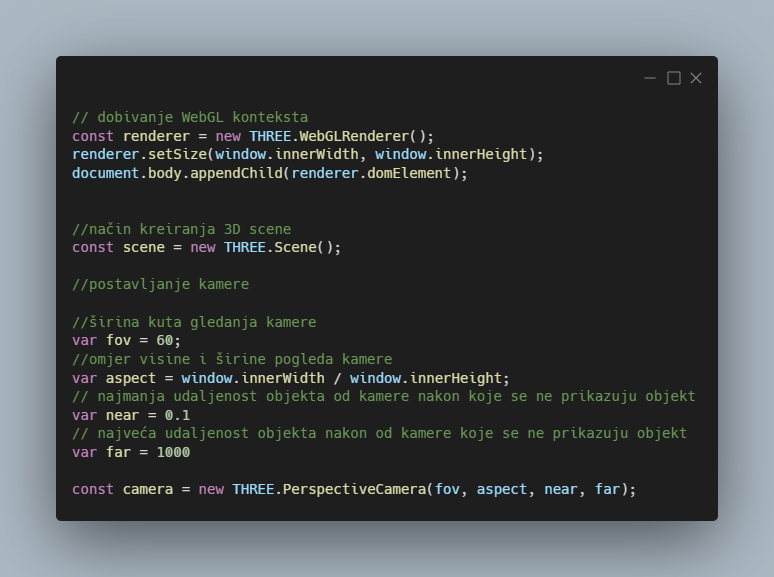
\includegraphics[scale=0.5]{image/zadatak1.png}
    \caption{Primjer koda za postavljanje kamere.}
\end{figure}


Dakle kao što vidimo na slici 3D scena se kreira na Three.Scene() funkcijom. Da bi smo postavili kameru trebamo koristiti četiri varijable, a to su 
varijabla \textit{fov} koja se koristi za širinu kuta gledanja, \textit{aspect} za omjer visine i širine pogleda pomoću ugrađenih objekata browsera, \textit{near} je 
varijabla koja se koristi za predstavljanje najmanje udaljenosti gdje se objekt ne prikazuje na kameri te varijabla \textit{far} koja je predstavljanje najveću 
udaljenost gdje se objekt ne prikazuje na kameri.
varijabla \textit{camera} služi tome da se prije navedene četiri varijable stave kao parametri u funkciju \texttt{PerspectiveCamera}.
\subsection{Kreiranje scene i objekta}
\begin{figure}[ht]
    \centering
    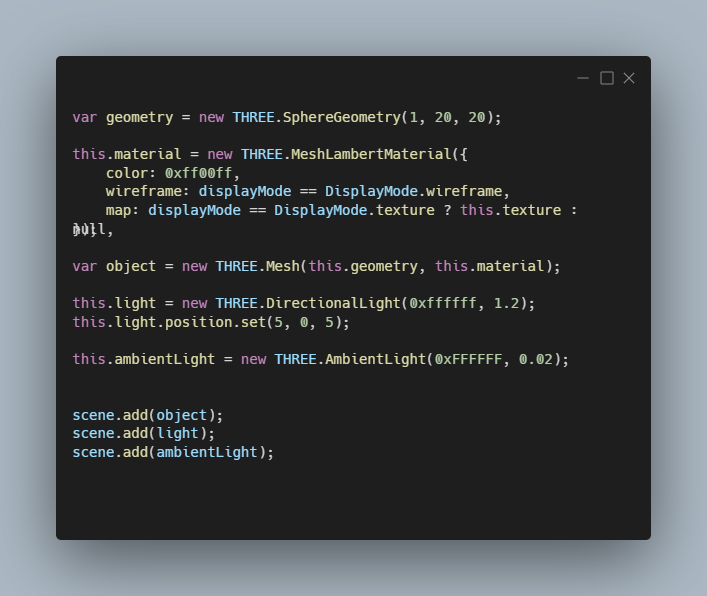
\includegraphics[scale=0.5]{image/zadatak1_objekti.png}
    \caption{Primjer koda za dodavanje objekta sceni te postavljanje svijetlosti i materijala.}
\end{figure}


Da bi smo dodali objekt u scenu moramo napraviti varijablu \textit{object} koja je predstavlja fukciju \texttt{Mesh}. \texttt{Mesh} je funkcija koja poprima dva parametra, a to su materijal i 
vrstu geometrijskog tijela. U kodu na slici se radi o sferi pa se prvo mora stvoriti varijabla \textit{geometry} koja predstavlja funkciju \texttt{SphereGeometry} koja stvara sferu.
Drugi parametar funkcije \texttt{Mesh} je material. \textit{Material} je također varijabla koja predstavlja funkciju \texttt{MeshLamberMaterial} koja stvara materijal prema određenoj boji, 
prikazu i teksturi. Kada smo to sve napravili tada možemo pozvati \texttt{add} funkciju da stvorimo objekt. Svijetlo  se također postavlja sa \texttt{add}.
Varijabla \textit{light} predstavlja funkciju \texttt{DirectionalLight} koja stvara svijetlost te tu svijetlost postavljamo na neku poziciju. 
\pagebreak
\subsection{Interakcija miša i tastature s scenom.}
\begin{figure}[ht]
    \centering
    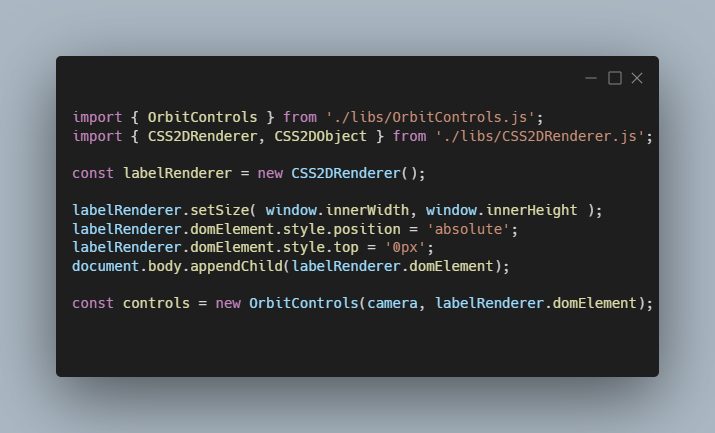
\includegraphics[scale=0.5]{image/zadatak1_kontrole.png}
    \caption{Primjer koda za interakciju miša i tastature s scenom.}
\end{figure}

Interakcija preko miša i tastature se implementira se postiže sa objektima OrbitControls i renderer. Orbit controls omogućava da se kamera kreće oko modela,
a CSS2DRenderer prikazuje sve potrebne elemente modela.

\pagebreak
\section{Zadatak 2.}

\subsection{Matematički model mrežastog prikaza za valjak}
\begin{flushleft}
    \begin{tabular}{||c | c | c ||} 
     \hline
     edge & start & end \\ [0.5ex] 
     \hline\hline
     1 & 6 & 87837  \\ 
     \hline
     2 & 7 & 78  \\
     \hline
     3 & 545 & 778  \\
     \hline
     4 & 545 & 18744 \\
     \hline
     5 & 88 & 788  \\ [1ex] 
     \hline
    \end{tabular}
    \end{flushleft}

    \subsection{Matematički model mrežastog prikaza za stošca}
\begin{flushleft}
    \begin{tabular}{||c | c | c ||} 
     \hline
     edge & start & end \\ [0.5ex] 
     \hline\hline
     1 & 6 & 87837  \\ 
     \hline
     2 & 7 & 78  \\
     \hline
     3 & 545 & 778  \\
     \hline
     4 & 545 & 18744 \\
     \hline
     5 & 88 & 788  \\ [1ex] 
     \hline
    \end{tabular}
    \end{flushleft}

    \subsection{Matematički model mrežastog prikaza za sfere}
\begin{flushleft}
    \begin{tabular}{||c | c | c ||} 
     \hline
     edge & start & end \\ [0.5ex] 
     \hline\hline
     1 & 6 & 87837  \\ 
     \hline
     2 & 7 & 78  \\
     \hline
     3 & 545 & 778  \\
     \hline
     4 & 545 & 18744 \\
     \hline
     5 & 88 & 788  \\ [1ex] 
     \hline
    \end{tabular}
    \end{flushleft}

\newpage
\subsection{Phongov model osvjetljenja}
Model se zasniva na podacima te se koristi za predviđanje ponašanja sustava, tzv empirijski model. Koristi se kod lokalnog osvjetljenja točke na nekoj površini.

\pagebreak
\section{Aplet}
Cilj apleta je vizualno ilustrirati definiciju kardioide. Opišimo ukratko funkcioniranje apleta: BLA BLA BLA BLA

\LaTeX{} može ubaciti vanjsku sliku u svoj dokument. Slika pritom mora biti u odgovarajućem formatu i najjednostavnije je da se nalazi u tekućem
direktoriju \verb|tex| datoteke. Nadalje, \LaTeX{} ima dosta svojih fantastičnih paketa za crtanje slika kao što je \verb|tikz| paket.\par
\vspace*{5mm}
\begin{figure}[!h]
\centering

\caption{Kardioida u \texttt{GeoGebri}}
\end{figure}

\paragraph{Referenciranje na literaturu.} Prema literaturi \cite{Maric} vrijedi\,\ldots \ Prema literaturi \cite{geo} mora biti\,\ldots

\begin{thebibliography}{9}

\bibitem{Youtube} Jeff Anderson \emph{Applied Linear Algebra, Lesson 7, Video 5: Wireframe Model in 3D} \texttt{https://www.youtube.com/watch?v=FDDl5PQBAkM} (3.1.2023.)
\bibitem{Youtube} Jeff Anderson \emph{Applied Linear Algebra, Lesson 7, Video 6: Wireframe Model in 3D} \texttt{https://www.youtube.com/watch?v=6KJH1dG8qLY} (3.1.2023.)
\bibitem{Youtube} Jeff Anderson \emph{Applied Linear Algebra, Lesson 7, Video 7: Wireframe Model in 3D} \texttt{https://www.youtube.com/watch?v=YaxuxZiXnKI} (3.1.2023.)
\bibitem{geo} Three.js, \texttt{https://threejs.org/}, (28.12.2022.)
\bibitem{geo} GeoGebra, \texttt{http://www.geogebra.org/cms/}, (4.1.2023.)
\end{thebibliography}

\end{document}